%% bare_conf.tex
%% V1.4b
%% 2015/08/26
%% by Michael Shell
%% See:
%% http://www.michaelshell.org/
%% for current contact information.
%%
%% This is a skeleton file demonstrating the use of IEEEtran.cls
%% (requires IEEEtran.cls version 1.8b or later) with an IEEE
%% conference paper.
%%
%% Support sites:
%% http://www.michaelshell.org/tex/ieeetran/
%% http://www.ctan.org/pkg/ieeetran
%% and
%% http://www.ieee.org/

%%*************************************************************************
%% Legal Notice:
%% This code is offered as-is without any warranty either expressed or
%% implied; without even the implied warranty of MERCHANTABILITY or
%% FITNESS FOR A PARTICULAR PURPOSE! 
%% User assumes all risk.
%% In no event shall the IEEE or any contributor to this code be liable for
%% any damages or losses, including, but not limited to, incidental,
%% consequential, or any other damages, resulting from the use or misuse
%% of any information contained here.
%%
%% All comments are the opinions of their respective authors and are not
%% necessarily endorsed by the IEEE.
%%
%% This work is distributed under the LaTeX Project Public License (LPPL)
%% ( http://www.latex-project.org/ ) version 1.3, and may be freely used,
%% distributed and modified. A copy of the LPPL, version 1.3, is included
%% in the base LaTeX documentation of all distributions of LaTeX released
%% 2003/12/01 or later.
%% Retain all contribution notices and credits.
%% ** Modified files should be clearly indicated as such, including  **
%% ** renaming them and changing author support contact information. **
%%*************************************************************************


% *** Authors should verify (and, if needed, correct) their LaTeX system  ***
% *** with the testflow diagnostic prior to trusting their LaTeX platform ***
% *** with production work. The IEEE's font choices and paper sizes can   ***
% *** trigger bugs that do not appear when using other class files.       ***                          ***
% The testflow support page is at:
% http://www.michaelshell.org/tex/testflow/



\documentclass[conference]{IEEEtran}
% Some Computer Society conferences also require the compsoc mode option,
% but others use the standard conference format.
%
% If IEEEtran.cls has not been installed into the LaTeX system files,
% manually specify the path to it like:
% \documentclass[conference]{../sty/IEEEtran}





% Some very useful LaTeX packages include:
% (uncomment the ones you want to load)


% *** MISC UTILITY PACKAGES ***
%
%\usepackage{ifpdf}
% Heiko Oberdiek's ifpdf.sty is very useful if you need conditional
% compilation based on whether the output is pdf or dvi.
% usage:
% \ifpdf
%   % pdf code
% \else
%   % dvi code
% \fi
% The latest version of ifpdf.sty can be obtained from:
% http://www.ctan.org/pkg/ifpdf
% Also, note that IEEEtran.cls V1.7 and later provides a builtin
% \ifCLASSINFOpdf conditional that works the same way.
% When switching from latex to pdflatex and vice-versa, the compiler may
% have to be run twice to clear warning/error messages.






% *** CITATION PACKAGES ***
%
%\usepackage{cite}
% cite.sty was written by Donald Arseneau
% V1.6 and later of IEEEtran pre-defines the format of the cite.sty package
% \cite{} output to follow that of the IEEE. Loading the cite package will
% result in citation numbers being automatically sorted and properly
% "compressed/ranged". e.g., [1], [9], [2], [7], [5], [6] without using
% cite.sty will become [1], [2], [5]--[7], [9] using cite.sty. cite.sty's
% \cite will automatically add leading space, if needed. Use cite.sty's
% noadjust option (cite.sty V3.8 and later) if you want to turn this off
% such as if a citation ever needs to be enclosed in parenthesis.
% cite.sty is already installed on most LaTeX systems. Be sure and use
% version 5.0 (2009-03-20) and later if using hyperref.sty.
% The latest version can be obtained at:
% http://www.ctan.org/pkg/cite
% The documentation is contained in the cite.sty file itself.






% *** GRAPHICS RELATED PACKAGES ***
%
\ifCLASSINFOpdf
  % \usepackage[pdftex]{graphicx}
  % declare the path(s) where your graphic files are
  % \graphicspath{{../pdf/}{../jpeg/}}
  % and their extensions so you won't have to specify these with
  % every instance of \includegraphics
  % \DeclareGraphicsExtensions{.pdf,.jpeg,.png}
\else
  % or other class option (dvipsone, dvipdf, if not using dvips). graphicx
  % will default to the driver specified in the system graphics.cfg if no
  % driver is specified.
  % \usepackage[dvips]{graphicx}
  % declare the path(s) where your graphic files are
  % \graphicspath{{../eps/}}
  % and their extensions so you won't have to specify these with
  % every instance of \includegraphics
  % \DeclareGraphicsExtensions{.eps}
\fi
% graphicx was written by David Carlisle and Sebastian Rahtz. It is
% required if you want graphics, photos, etc. graphicx.sty is already
% installed on most LaTeX systems. The latest version and documentation
% can be obtained at: 
% http://www.ctan.org/pkg/graphicx
% Another good source of documentation is "Using Imported Graphics in
% LaTeX2e" by Keith Reckdahl which can be found at:
% http://www.ctan.org/pkg/epslatex
%
% latex, and pdflatex in dvi mode, support graphics in encapsulated
% postscript (.eps) format. pdflatex in pdf mode supports graphics
% in .pdf, .jpeg, .png and .mps (metapost) formats. Users should ensure
% that all non-photo figures use a vector format (.eps, .pdf, .mps) and
% not a bitmapped formats (.jpeg, .png). The IEEE frowns on bitmapped formats
% which can result in "jaggedy"/blurry rendering of lines and letters as
% well as large increases in file sizes.
%
% You can find documentation about the pdfTeX application at:
% http://www.tug.org/applications/pdftex





% *** MATH PACKAGES ***
%
%\usepackage{amsmath}
% A popular package from the American Mathematical Society that provides
% many useful and powerful commands for dealing with mathematics.
%
% Note that the amsmath package sets \interdisplaylinepenalty to 10000
% thus preventing page breaks from occurring within multiline equations. Use:
%\interdisplaylinepenalty=2500
% after loading amsmath to restore such page breaks as IEEEtran.cls normally
% does. amsmath.sty is already installed on most LaTeX systems. The latest
% version and documentation can be obtained at:
% http://www.ctan.org/pkg/amsmath





% *** SPECIALIZED LIST PACKAGES ***
%
%\usepackage{algorithmic}
% algorithmic.sty was written by Peter Williams and Rogerio Brito.
% This package provides an algorithmic environment fo describing algorithms.
% You can use the algorithmic environment in-text or within a figure
% environment to provide for a floating algorithm. Do NOT use the algorithm
% floating environment provided by algorithm.sty (by the same authors) or
% algorithm2e.sty (by Christophe Fiorio) as the IEEE does not use dedicated
% algorithm float types and packages that provide these will not provide
% correct IEEE style captions. The latest version and documentation of
% algorithmic.sty can be obtained at:
% http://www.ctan.org/pkg/algorithms
% Also of interest may be the (relatively newer and more customizable)
% algorithmicx.sty package by Szasz Janos:
% http://www.ctan.org/pkg/algorithmicx




% *** ALIGNMENT PACKAGES ***
%
%\usepackage{array}
% Frank Mittelbach's and David Carlisle's array.sty patches and improves
% the standard LaTeX2e array and tabular environments to provide better
% appearance and additional user controls. As the default LaTeX2e table
% generation code is lacking to the point of almost being broken with
% respect to the quality of the end results, all users are strongly
% advised to use an enhanced (at the very least that provided by array.sty)
% set of table tools. array.sty is already installed on most systems. The
% latest version and documentation can be obtained at:
% http://www.ctan.org/pkg/array


% IEEEtran contains the IEEEeqnarray family of commands that can be used to
% generate multiline equations as well as matrices, tables, etc., of high
% quality.




% *** SUBFIGURE PACKAGES ***
%\ifCLASSOPTIONcompsoc
%  \usepackage[caption=false,font=normalsize,labelfont=sf,textfont=sf]{subfig}
%\else
%  \usepackage[caption=false,font=footnotesize]{subfig}
%\fi
% subfig.sty, written by Steven Douglas Cochran, is the modern replacement
% for subfigure.sty, the latter of which is no longer maintained and is
% incompatible with some LaTeX packages including fixltx2e. However,
% subfig.sty requires and automatically loads Axel Sommerfeldt's caption.sty
% which will override IEEEtran.cls' handling of captions and this will result
% in non-IEEE style figure/table captions. To prevent this problem, be sure
% and invoke subfig.sty's "caption=false" package option (available since
% subfig.sty version 1.3, 2005/06/28) as this is will preserve IEEEtran.cls
% handling of captions.
% Note that the Computer Society format requires a larger sans serif font
% than the serif footnote size font used in traditional IEEE formatting
% and thus the need to invoke different subfig.sty package options depending
% on whether compsoc mode has been enabled.
%
% The latest version and documentation of subfig.sty can be obtained at:
% http://www.ctan.org/pkg/subfig




% *** FLOAT PACKAGES ***
%
%\usepackage{fixltx2e}
% fixltx2e, the successor to the earlier fix2col.sty, was written by
% Frank Mittelbach and David Carlisle. This package corrects a few problems
% in the LaTeX2e kernel, the most notable of which is that in current
% LaTeX2e releases, the ordering of single and double column floats is not
% guaranteed to be preserved. Thus, an unpatched LaTeX2e can allow a
% single column figure to be placed prior to an earlier double column
% figure.
% Be aware that LaTeX2e kernels dated 2015 and later have fixltx2e.sty's
% corrections already built into the system in which case a warning will
% be issued if an attempt is made to load fixltx2e.sty as it is no longer
% needed.
% The latest version and documentation can be found at:
% http://www.ctan.org/pkg/fixltx2e


%\usepackage{stfloats}
% stfloats.sty was written by Sigitas Tolusis. This package gives LaTeX2e
% the ability to do double column floats at the bottom of the page as well
% as the top. (e.g., "\begin{figure*}[!b]" is not normally possible in
% LaTeX2e). It also provides a command:
%\fnbelowfloat
% to enable the placement of footnotes below bottom floats (the standard
% LaTeX2e kernel puts them above bottom floats). This is an invasive package
% which rewrites many portions of the LaTeX2e float routines. It may not work
% with other packages that modify the LaTeX2e float routines. The latest
% version and documentation can be obtained at:
% http://www.ctan.org/pkg/stfloats
% Do not use the stfloats baselinefloat ability as the IEEE does not allow
% \baselineskip to stretch. Authors submitting work to the IEEE should note
% that the IEEE rarely uses double column equations and that authors should try
% to avoid such use. Do not be tempted to use the cuted.sty or midfloat.sty
% packages (also by Sigitas Tolusis) as the IEEE does not format its papers in
% such ways.
% Do not attempt to use stfloats with fixltx2e as they are incompatible.
% Instead, use Morten Hogholm'a dblfloatfix which combines the features
% of both fixltx2e and stfloats:
%
% \usepackage{dblfloatfix}
% The latest version can be found at:
% http://www.ctan.org/pkg/dblfloatfix




% *** PDF, URL AND HYPERLINK PACKAGES ***
%
%\usepackage{url}
% url.sty was written by Donald Arseneau. It provides better support for
% handling and breaking URLs. url.sty is already installed on most LaTeX
% systems. The latest version and documentation can be obtained at:
% http://www.ctan.org/pkg/url
% Basically, \url{my_url_here}.




% *** Do not adjust lengths that control margins, column widths, etc. ***
% *** Do not use packages that alter fonts (such as pslatex).         ***
% There should be no need to do such things with IEEEtran.cls V1.6 and later.
% (Unless specifically asked to do so by the journal or conference you plan
% to submit to, of course. )


% correct bad hyphenation here
\hyphenation{op-tical net-works semi-conduc-tor}

\usepackage{graphicx}
\usepackage{booktabs}
\usepackage{multicol}
\usepackage{multirow}
\usepackage{diagbox} % 加载宏包
\usepackage{amsmath}

% 表格
\usepackage[utf8]{inputenc}
\usepackage{fourier} 
\usepackage{array}
\usepackage{makecell}

\renewcommand\theadalign{bc}
\renewcommand\theadfont{\bfseries}
\renewcommand\theadgape{\Gape[4pt]}
\renewcommand\cellgape{\Gape[4pt]}

\begin{document}
%
% paper title
% Titles are generally capitalized except for words such as a, an, and, as,
% at, but, by, for, in, nor, of, on, or, the, to and up, which are usually
% not capitalized unless they are the first or last word of the title.
% Linebreaks \\ can be used within to get better formatting as desired.
% Do not put math or special symbols in the title.
\title{Deep Learning for Network Intrusion Detection}


% author names and affiliations
% use a multiple column layout for up to three different
% affiliations
\author{\IEEEauthorblockN{Zhikai Chen, Xinyu Cai, Zhipeng Huang}
\IEEEauthorblockA{
% PB16051320 \\
School of Information Science and Technology\\
University of Science and Technology of China\\
\{czk654, cxyvlf, hzp1104\}@mail.ustc.edu.cn}
}

% conference papers do not typically use \thanks and this command
% is locked out in conference mode. If really needed, such as for
% the acknowledgment of grants, issue a \IEEEoverridecommandlockouts
% after \documentclass

% for over three affiliations, or if they all won't fit within the width
% of the page, use this alternative format:
% 
%\author{\IEEEauthorblockN{Michael Shell\IEEEauthorrefmark{1},
%Homer Simpson\IEEEauthorrefmark{2},
%James Kirk\IEEEauthorrefmark{3}, 
%Montgomery Scott\IEEEauthorrefmark{3} and
%Eldon Tyrell\IEEEauthorrefmark{4}}
%\IEEEauthorblockA{\IEEEauthorrefmark{1}School of Electrical and Computer Engineering\\
%Georgia Institute of Technology,
%Atlanta, Georgia 30332--0250\\ Email: see http://www.michaelshell.org/contact.html}
%\IEEEauthorblockA{\IEEEauthorrefmark{2}Twentieth Century Fox, Springfield, USA\\
%Email: homer@thesimpsons.com}
%\IEEEauthorblockA{\IEEEauthorrefmark{3}Starfleet Academy, San Francisco, California 96678-2391\\
%Telephone: (800) 555--1212, Fax: (888) 555--1212}
%\IEEEauthorblockA{\IEEEauthorrefmark{4}Tyrell Inc., 123 Replicant Street, Los Angeles, California 90210--4321}}




% use for special paper notices
%\IEEEspecialpapernotice{(Invited Paper)}




% make the title area
\maketitle

% As a general rule, do not put math, special symbols or citations
% in the abstract
\begin{abstract}
Network Intrusion Detection System (NIDS) monitors the running state of a network to detect attacking attempts, behaviors and results, for the sake of protecting the network system's confidentiality, integrity and availability.

In this paper, we focus on intrusion detection system in the network security instead of computer (host) security and summarize the recent deep learning methods in particular for characteristics of internet environment, then propose our assumed approaches and rising prospects for further research in Deep Learning for Cyber-security.
\end{abstract}

% no keywords




% For peer review papers, you can put extra information on the cover
% page as needed:
% \ifCLASSOPTIONpeerreview
% \begin{center} \bfseries EDICS Category: 3-BBND \end{center}
% \fi
%
% For peerreview papers, this IEEEtran command inserts a page break and
% creates the second title. It will be ignored for other modes.
\IEEEpeerreviewmaketitle



\section{Introduction}
% no \IEEEPARstart
Cyber-security is the practice of protecting systems, networks, and programs from digital attacks. These cyber-attacks are usually aimed at accessing, changing, or destroying sensitive information; extorting money from users; or interrupting normal business processes. Implementing effective cyber-security measures is particularly challenging today because there are more devices than people, and attackers are becoming more innovative. Intrusion detection system (IDS) plays a necessary role in network security in order to discover, determine, and identify unauthorized usage, duplication, alteration, and destruction of information systems[1]. By collecting key information from a computer network and analyzing it, it is possible to discover whether there are violations of security policies and signs of attacks in the networks. 

There are three main types of cyber analysis in support of NIDS: misuse-based, anomaly-based and hybrid. Misused-based methods aim at collecting the illegal operations in networks and building a database for attacks, then it is able to match the characteristics of known attacks automatically for behaviors to detect intrusion among them. However, they are not pretty appropriate especially for some complex environments of networks nowadays partly because the frequent manual updates of database and the lack of intrusion connections, which limits the capability of these methods to capture their features. Anomaly detection techniques such as Isolation Forest can handle the imbalanced data, which uses plenty of normal network activities to model the profiles of normal network. With their ability to detect novel attacks and existed datasets, they become popular with learning-based methods recently since detection can be regarded as a classification problem for either raw traffic data, packets or their features.

From the perspective of artificial intelligence (AI) development, traditional port-based and deep packets inspection (DPI)-based methods are rule-based approaches, which perform classification by matching predefined hard-coded rules. Statistical-based and behavioral-based methods are classic machine learning (ML) approaches, which classify traffic by extracting patterns from empirical data using a set of selective features. 

A simple definition states that Deep Learning (DL) is a set of machine learning algorithms that attempt to learn in multiple levels, corresponding to different levels of abstraction. The levels correspond to distinct levels of concepts, where higher-level concepts are defined from and helped lower-level ones. Feature extraction is performed by the first few layers of the deep network. There are unsupervised, supervised, and hybrid DL architectures. Because shallow neural networks have only one hidden layer, they lack the ability to perform advanced and unable to learn high-level concepts as deep neural networks. This also holds true for other machine learning algorithms, as well. Deep learning algorithms well capture the intrusion features and packets data distribution and it becomes possible to update automatically the model's parameters according to the situation in complex networks environment while there are unknown data packets. Further more, these methods usually need no hand-designed features but directly took raw traffic as input data of classifier which is representation learning different from rule-based or classic ML approaches as shown in Fig. \ref{fig:3m} As the development of effective DL methods and collection of various data set, it has achieved state-of-the-art performance in different experiments and derived a series of network intrusion detection system.

This work can be generally divided into three parts. (i) We introduce the datasets generally used in deep learning methods for intrusion detection and the metrics to evaluate the discriminate model. (ii) We illustrate the thesis and significant components of recent influential works in this field, including deep belief networks (DBN), autoencoder or variant autoencoder (VAE), convolution neural networks (CNN), recurrent neural networks (RNN) or long-short term memory networks (LSTM) and generative adversarial networks (GAN) utilized in intrusion detection for different application. (iii) We assume some methods in two different perspectives for future improvement, including a means to improve the  present limitation such as high false detection rate of anomaly detection and imbalanced data for some attacking classes and an application of a potential and feasible framework for intrusion detection in a series of data packets based on long-term recurrent convolutional networks with images analysis. 

\begin{figure}[ht]
\centering
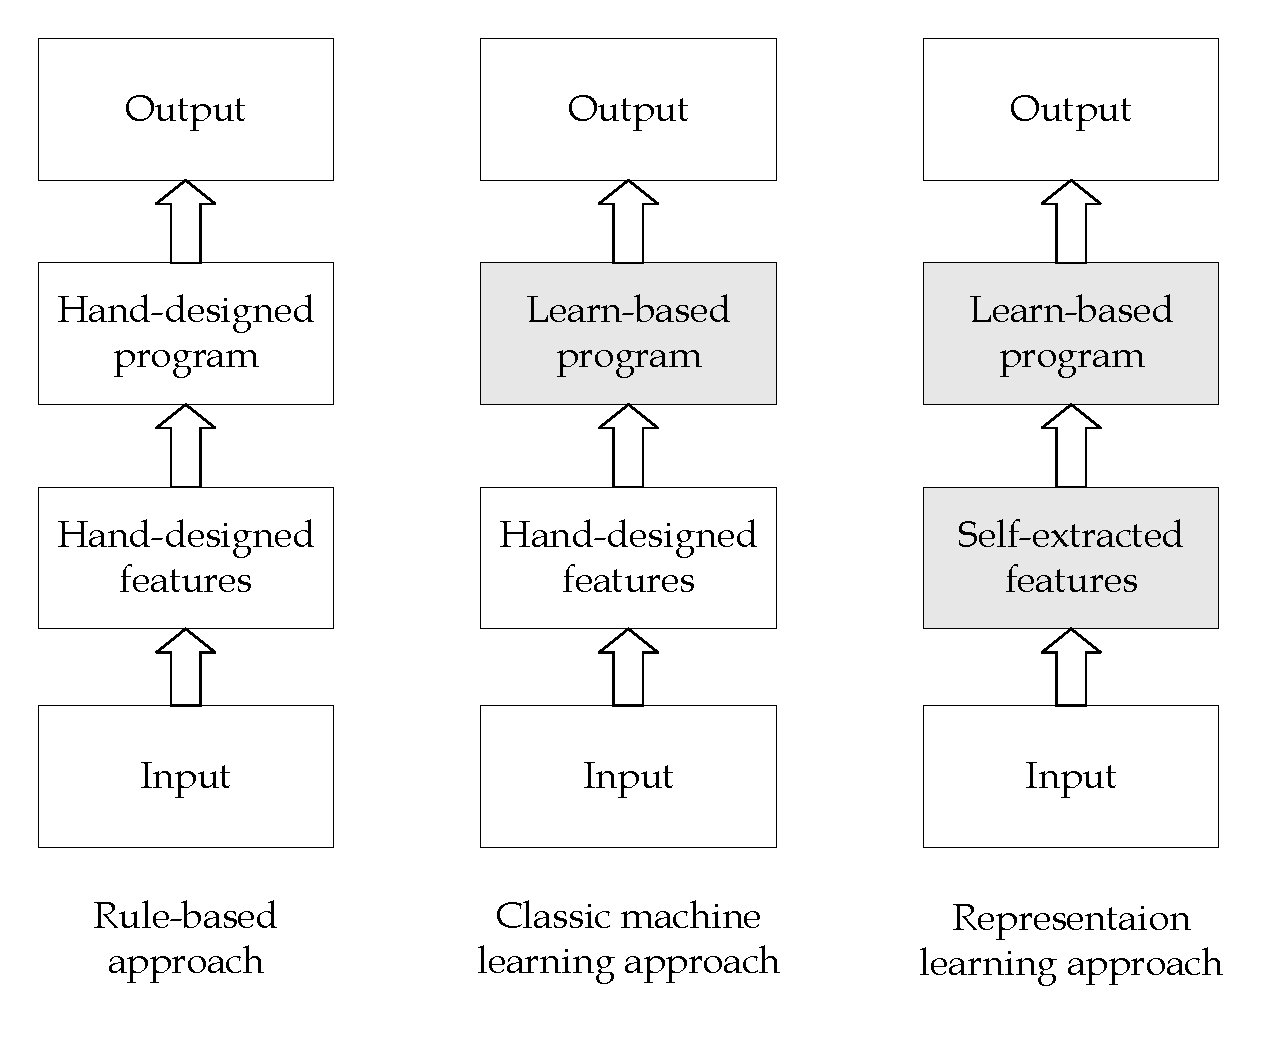
\includegraphics[scale=0.4]{pictures/3m.pdf}
\caption{Work flows of traffic classification}
\label{fig:3m}
\end{figure}
% You must have at least 2 lines in the paragraph with the drop letter
% (should never be an issue)

 
\hfill May 28, 2019

% An example of a floating figure using the graphicx package.
% Note that \label must occur AFTER (or within) \caption.
% For figures, \caption should occur after the \includegraphics.
% Note that IEEEtran v1.7 and later has special internal code that
% is designed to preserve the operation of \label within \caption
% even when the captionsoff option is in effect. However, because
% of issues like this, it may be the safest practice to put all your
% \label just after \caption rather than within \caption{}.
%
% Reminder: the "draftcls" or "draftclsnofoot", not "draft", class
% option should be used if it is desired that the figures are to be
% displayed while in draft mode.
%
%\begin{figure}[!t]
%\centering
%\includegraphics[width=2.5in]{myfigure}
% where an .eps filename suffix will be assumed under latex, 
% and a .pdf suffix will be assumed for pdflatex; or what has been declared
% via \DeclareGraphicsExtensions.
%\caption{Simulation results for the network.}
%\label{fig_sim}
%\end{figure}

% Note that the IEEE typically puts floats only at the top, even when this
% results in a large percentage of a column being occupied by floats.


% An example of a double column floating figure using two subfigures.
% (The subfig.sty package must be loaded for this to work.)
% The subfigure \label commands are set within each subfloat command,
% and the \label for the overall figure must come after \caption.
% \hfil is used as a separator to get equal spacing.
% Watch out that the combined width of all the subfigures on a 
% line do not exceed the text width or a line break will occur.
%
%\begin{figure*}[!t]
%\centering
%\subfloat[Case I]{\includegraphics[width=2.5in]{box}%
%\label{fig_first_case}}
%\hfil
%\subfloat[Case II]{\includegraphics[width=2.5in]{box}%
%\label{fig_second_case}}
%\caption{Simulation results for the network.}
%\label{fig_sim}
%\end{figure*}
%
% Note that often IEEE papers with subfigures do not employ subfigure
% captions (using the optional argument to \subfloat[]), but instead will
% reference/describe all of them (a), (b), etc., within the main caption.
% Be aware that for subfig.sty to generate the (a), (b), etc., subfigure
% labels, the optional argument to \subfloat must be present. If a
% subcaption is not desired, just leave its contents blank,
% e.g., \subfloat[].


% An example of a floating table. Note that, for IEEE style tables, the
% \caption command should come BEFORE the table and, given that table
% captions serve much like titles, are usually capitalized except for words
% such as a, an, and, as, at, but, by, for, in, nor, of, on, or, the, to
% and up, which are usually not capitalized unless they are the first or
% last word of the caption. Table text will default to \footnotesize as
% the IEEE normally uses this smaller font for tables.
% The \label must come after \caption as always.
%
%\begin{table}[!t]
%% increase table row spacing, adjust to taste
%\renewcommand{\arraystretch}{1.3}
% if using array.sty, it might be a good idea to tweak the value of
% \extrarowheight as needed to properly center the text within the cells
%\caption{An Example of a Table}
%\label{table_example}
%\centering
%% Some packages, such as MDW tools, offer better commands for making tables
%% than the plain LaTeX2e tabular which is used here.
%\begin{tabular}{|c||c|}
%\hline
%One & Two\\
%\hline
%Three & Four\\
%\hline
%\end{tabular}
%\end{table}


% Note that the IEEE does not put floats in the very first column
% - or typically anywhere on the first page for that matter. Also,
% in-text middle ("here") positioning is typically not used, but it
% is allowed and encouraged for Computer Society conferences (but
% not Computer Society journals). Most IEEE journals/conferences use
% top floats exclusively. 
% Note that, LaTeX2e, unlike IEEE journals/conferences, places
% footnotes above bottom floats. This can be corrected via the
% \fnbelowfloat command of the stfloats package.
\section{Evaluation}

\subsection{Metrics}

This section describes several classification metrics used by traditional valuation. For a model performing a binary classification task, there are a number of different metrics. Accuracy, precision, recall, false positive rate, F1 Score, and area under curve (AUC) are included and many of the metrics have more than one name. All of these evaluation metrics are derived from the four values found in the confusion matrix (Table \ref{tab:metrics}), which is based on the calculated predicted class versus the actual class (ground truth).

\begin{table}[!htbp]
\centering
\caption{Confusion matrix}
\begin{tabular}{|c|c|c|}
\hline
\diagbox{Actual}{Predicted}  &Malicious    &Benign \\ %添加斜线表头
\hline
Malicious  &True Positive (TP)  &False Negative (FN)\\
\hline
Benign  &False Positive (FP)   &True Negative (TN) \\
\hline
\end{tabular}
\label{tab:metrics}
\end{table}

Accuracy  (acc)  or  Proportion  Correct:  the  ratio  of  correctly  classified  examples  to  all  items.The usefulness of accuracy is lower when the classes are unbalanced (i.e., there are a significantly larger number of examples from one class than from another). However, it does provide useful insight when the classes are balanced.
\begin{equation}
a c c=\frac{T P+T N}{T P+T N+F P+F N}
\end{equation}
Positive Predictive Value (PPV) or Precision (p): The ratio of items correctly classified as class X total items that were classified as class X
\begin{equation}
p=\frac{T P}{T P+F P}
\end{equation}
Sensitivity or True Positive Rate (TPR) or Probability of Detection(PD)or Recall (r): The ratio of items correctly classified as X to all items that were actually class X.
\begin{equation}
T P R=\frac{T P}{T P+F N}
\end{equation}
Negative Predictive Value (NPV): The ratio of items correctly classified as not X to all items classified as not X.
\begin{equation}
N P V=\frac{T N}{T N+F N}
\end{equation}
Specificity or True Negative Rate (TNR): The ratio of items correctly classified as not X to all items that are not class X.
\begin{equation}
T N R=\frac{T N}{T N+F P}
\end{equation}
False Alarm Rate (FAR) or False Positive Rate (FPR) or Fall-Out: The ratio of items incorrectly classified as class X to all the items that are not class X.
\begin{equation}
F P R=\frac{F P}{T N+F P}
\end{equation}
F1 Score (F1): The F1 Score is the harmonic mean of the precision (p) and the true positive rate (r).
\begin{equation}
F_{1}=\frac{2}{\frac{1}{r}+\frac{1}{p}}=2 \frac{p * r}{p+r}
\end{equation}
This is a specific version of the F-$\beta$function, in which precision and true positive rate are given equal importance. 

Area under the curve (AUC): The sum of the area under a receiver operating characteristic (ROC) curve, which is a plot of the false positive rate versus the true positive rate, created by varying the classification thresholds. 

For multi-class problems, accuracy can be easily calculated; however, metrics such as precision, recall, FPR, F1 Score, and AUC cannot be calculated in a straightforward fashion (e.g., TP, TN do not exist for three-class problems).  Precision, recall, etc.  can be determined for a 3+ class problem by collapsing the problem into a two-class problem (i.e., all versus one), where the metrics are calculated for each class. Usually, the only accuracy is used for multiclass problems.

It is important to remember that because each of the papers described later uses a different dataset (or sometimes a different subset of a given dataset), it is not possible to compare the models developed based on the accuracy (or any other metrics) they obtained. Such a comparison would be valid only if the authors of both publications used exactly the same training dataset and the same testing dataset.

\begin{table}[!htbp]
\centering
\caption{ATTACKS WITHIN THE NETWORK-BASED DATA SETS}
\begin{tabular}{|c|c|}
\hline
\thead{Data Set}    &\thead{Attacks}    \\
\hline
\makecell{CIDDS-001}   &\makecell{DoS,  port  scans  (ping-scan, \\ SYN-Scan),  SSHbrute force} \\
\hline
\makecell{CIDDS-002}   &\makecell{port   scans   (ACK-Scan, \\  FIN-Scan,   ping-Scan,UDP-Scan, SYN-Scan)}  \\
\hline
\makecell{CTU-13}      &\makecell{botnets (Menti, Murlo, \\Neris, NSIS, Rbot,\\ Sogou,Virut)}  \\
\hline
\makecell{DARPA}       &\makecell{DoS, remote-to-local,\\ user-to-root, probing}    \\
\hline
\makecell{KDD CUP 99}  &\makecell{DoS, remote-to-local,\\ user-to-root, probing}    \\
\hline
\makecell{NSL-KDD}     &\makecell{DoS, remote-to-local,\\ user-to-root, probing}    \\
\hline

\end{tabular}
\label{tab:attackOnDataSet}
\end{table}

\subsection{Related Datasets}
An overview of some widely-used and significant datasets are shown in Fig. \ref{tab:attackOnDataSet}. Then we give an introduction of them one by one as follows. 

\subsubsection{DARPA 1998/1999}
The Defense Advanced Research Projects Agency (DARPA) 1998 \cite{lippmann2000evaluating} and DARPA 1999 data sets \cite{lippmann20001999} are extensively used in experiments and frequently cited in publications. The DARPA 1998 set was created by the Cyber Systems and Technology Group of the Massachusetts Institute of Technology Lincoln Laboratory (MIT/LL). DARPA 1999 data set had substantially more attack types than the DARPA 1998 data set. In both collections, the data sets were processed and curated to be used in the experiments. The TCP dumps and logs were combined into one stream with many columns. The data in DARPA dataset are tcp dump. Training data and test data are recorded for 5 million connections and 2 million connections. The dataset has 41 features such as protocol type, flag, duration, service etc and their descriptions. And 22 attacks such as DoS, Probe, U2R, R2L etc. are recorded in the dataset. DoS means denial-of-service. Probe is a surveillance attack. U2R is an attack which tries to unauthorized access to superuser. R2L is an unauthorized remote access attack.

\subsubsection{KDD 1999}
The Knowledge Discovery and Dissemination (KDD) 1999 dataset analyzed by \cite{tavallaee2009detailed} is one of the most widely used datasets for intrusion detection with about 4 million records of normal and attack traffic. There are a huge number of redundant records (78\% in the training data and 75\% in test data) causing bias. In addition, in the classification experiments the group conducted, they pointed out that by randomly selecting subsets of the training and testing data, often very high, unrealistic accuracies can be achieved. Therefore, Tavallaee et al. proposed a new data set, NSL-KDD, in order to overcome this shortcomings.

\subsubsection{CIDDS 001/002}
CIDDS (Coburg Intrusion Detection Data Sets) is a concept to create evaluation data sets for anomaly-based network intrusion detection systems. The CIDDS-001 data set was captured within an emulated small business environment in 2017, contains four weeks of unidirectional flow-based network traffic, and comes along with a detailed technical report with additional information. As a special feature, the data set encompasses an external server which was attacked in the internet. 

CIDDS-002 is a port scan data set which is created based on the scripts of CIDDS-001. The data set contains two weeks of unidirectional flow-based network traffic within an emulated small business environment. CIDDS-002 contains normal user behavior as well as a wide range of different port scan attacks. A technical report provides additional meta information about the data set where external IP addresses are anonymized. 


\subsubsection{CTU-13}
CTU-13 is the most commonly used dataset which contains raw packet data. The benefit of raw pcap files is the opportunity  for individuals to perform their own preprocessing, enabling a wider range of algorithms to be used. Additionally, the CTU-13 is not a simulated dataset. It contains 13 different scenarios with different numbers of computers and seven different botnet families. CTU-13 dataset and IXIA dataset compose USTC-TFC 2016 which contains 10 types of malicious data and 10 types of normal data. USTC-TFC 2016 is used to a CNN-based NIDS which will be illustrated in Section \ref{sec:cnn}.


\section{Recent Works}
Network intrusion detection systems are essential for ensuring the security of a network from various types of security breaches. There have been many approaches to intrusion detection using DL. We will explore them as follows.

\subsection{Deep Belief Networks}
Hinton et al. introduced Deep Belief Networks (DBNs) based on Restricted Boltzmann Machine (RBM) in \cite{hinton2006fast}. An RBM consists of the visible units and hidden units. The structure is shown in Fig. \ref{fig:rbm}. We use the vector $v$ and $h$ represent the visible units and the hidden unit state respectively. Then $v_i$ denotes the state of the i visible unit, $h_j$ denotes the state of the j hidden unit, $w, a_i, b_j$ are the weights between them and their bias respectively. They meet the energy formula \ref{eq:rbm_energy} as follows. With this structure, RBM can be trained in an unsupervised manner just with input for encoding or decoding. As a result, the weight updating rule as shown in formula \ref{eq:rbm_weight_update} go through a bidirectional propagation, where $\left\langle v_i h_j \right\rangle ^+$ indicates the average forward correlation and $\left\langle v_i h_j \right\rangle ^-$ indicates the average reverse correlation. $\epsilon$ denotes the learning rate.

\begin{equation}
\label{eq:rbm_energy}
E(v, h)=-\sum_{i \in V} b_{i} v_{i}-\sum_{j \in H} a_{j} h_{j}-\sum_{i, j} v_{i} h_{j} w_{i j}
\end{equation}

\begin{equation}
\begin{aligned}
w_{i j}(t+1) &= w_{i j}(t)+\Delta w_{i j}\\
&= w_{i j}(t)+\varepsilon\left(\left\langle v_{i} h_{j}\right\rangle^{+}-\left\langle v_{i} h_{j}\right\rangle^{-}\right)
\end{aligned}
\label{eq:rbm_weight_update}
\end{equation}

\begin{figure}[ht]
\centering
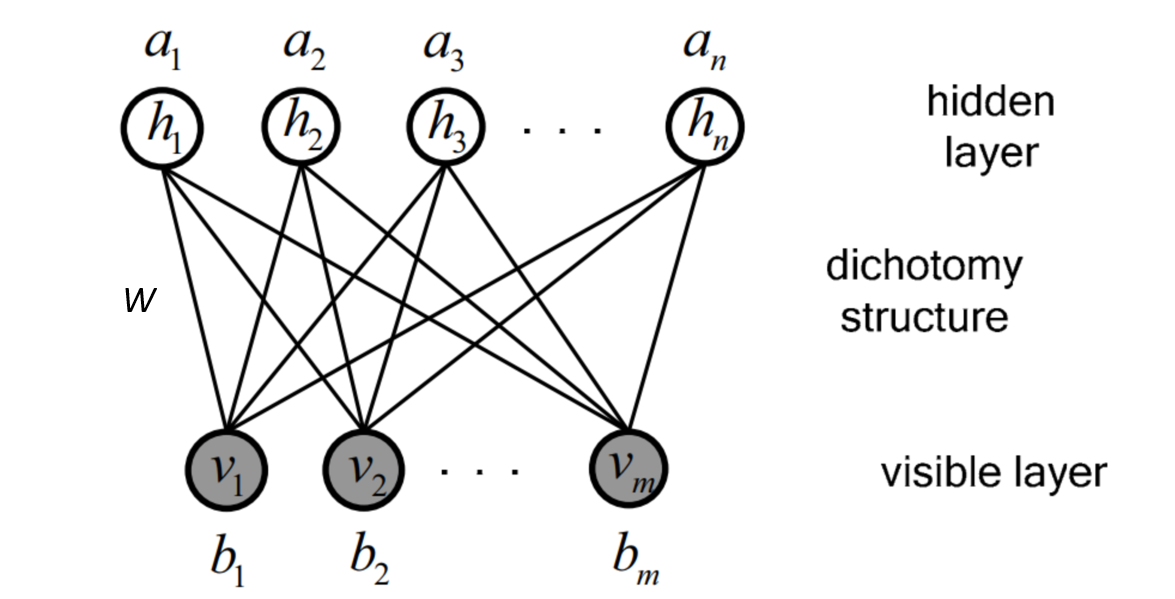
\includegraphics[scale=0.35]{pictures/RBM.PNG}
\caption{typical Restricted Boltzmann Machine}
\label{fig:rbm}
\end{figure}

DBNs are a class of deep neural networks composed of multiple layers of RBMs mentioned above and followed with a back propagation layers (BP) which can be a classification layer. RBMs are trained in an unsupervised manner. Typically each RBM layer in DBN is trained in unsupervised manner one after another, and finally train BP layer using back propagation in supervised manner.

Many network gateways and routers devices, which could potentially host a NIDS, do not have enough memory or processing power to train and sometimes even execute such model. Additionally, used in various situations and to detect numerous abnormal data packets, the parameters in a pretrained NIDS often need to be fine-tuned with current real-time data
after deployed to the network nodes.

A drawback of pure BP neural networks is that it needs a great amount of resources to train themselves, once begin training, the whole model is adjusted dramaticly.

Unlike traditional neural networks, DBNs' training process can be divided into two parts, pre-training and fine-tuning. Pre-training is processed in GPU and it generates an effective deep RBM which can refactor data and reduce data dimensions. After that, a two-level back-propagation network is added to it. The fine-tuning process on the network node only needs to adjust the last simple back-progradation network, which is a light, efficient and practical online manner and able to update the system from time to time.

\begin{figure}[ht]
\centering
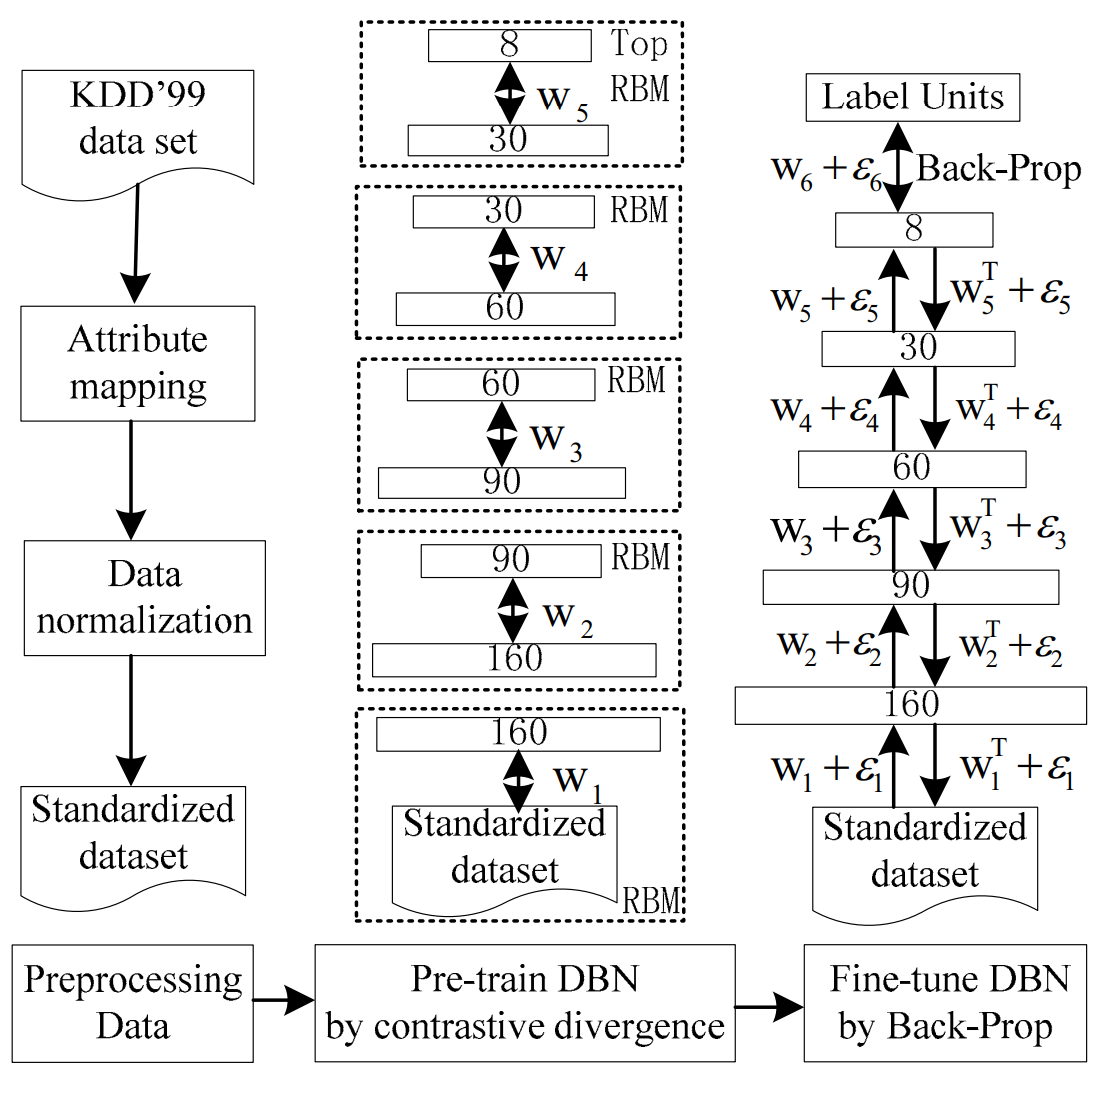
\includegraphics[scale=0.56]{pictures/DBN.PNG}
\caption{Deep Belief Network}
\label{fig:dbn}
\end{figure}

% DONE: what is and how to use DBN\\
% TO DO: why DBN, What to do with DBN

Gao et al. used a DBN for intrusion detection in \cite{gao2014intrusion} with KDD 1999 dataset. The best performing algorithm was a DBN with four hidden layers (six layers total), beating an SVM and DBNs with fewer layers. The accuracy was 93.49\%, with a TPR of 92.33\%. Nguyen et al. \cite{nguyen2018cyberattack} achieved similar accuracy using a similar architecture. Alrawashdeh and Purdy \cite{alrawashdeh2016toward} performed a similar experiment with a four-hidden-layer DBN and achieved an accuracy of 97.9\%. Alom et al. \cite{alom2015intrusion} built a similar model, but were able to achieve 97.5\% accuracy,training on 4\% of the data.

\subsection{Deep Autoencoders}
Autoencoders are a class of unsupervised neural networks composed of an encoder and a following decoder in which the network takes a vector as input and tries to match the output to that input vector. In another word, encoder is used to reconstruct the input to a hidden vector, and the decoder can recover the input vector from the hidden vector. Thus, the encoder can be used for dimension reduction by encoding or reconstructing the input, creating a higher or lower dimensionality representation of data. Typically, autoencoders are applied to extract the features of raw data.



\begin{figure}[ht]
\centering
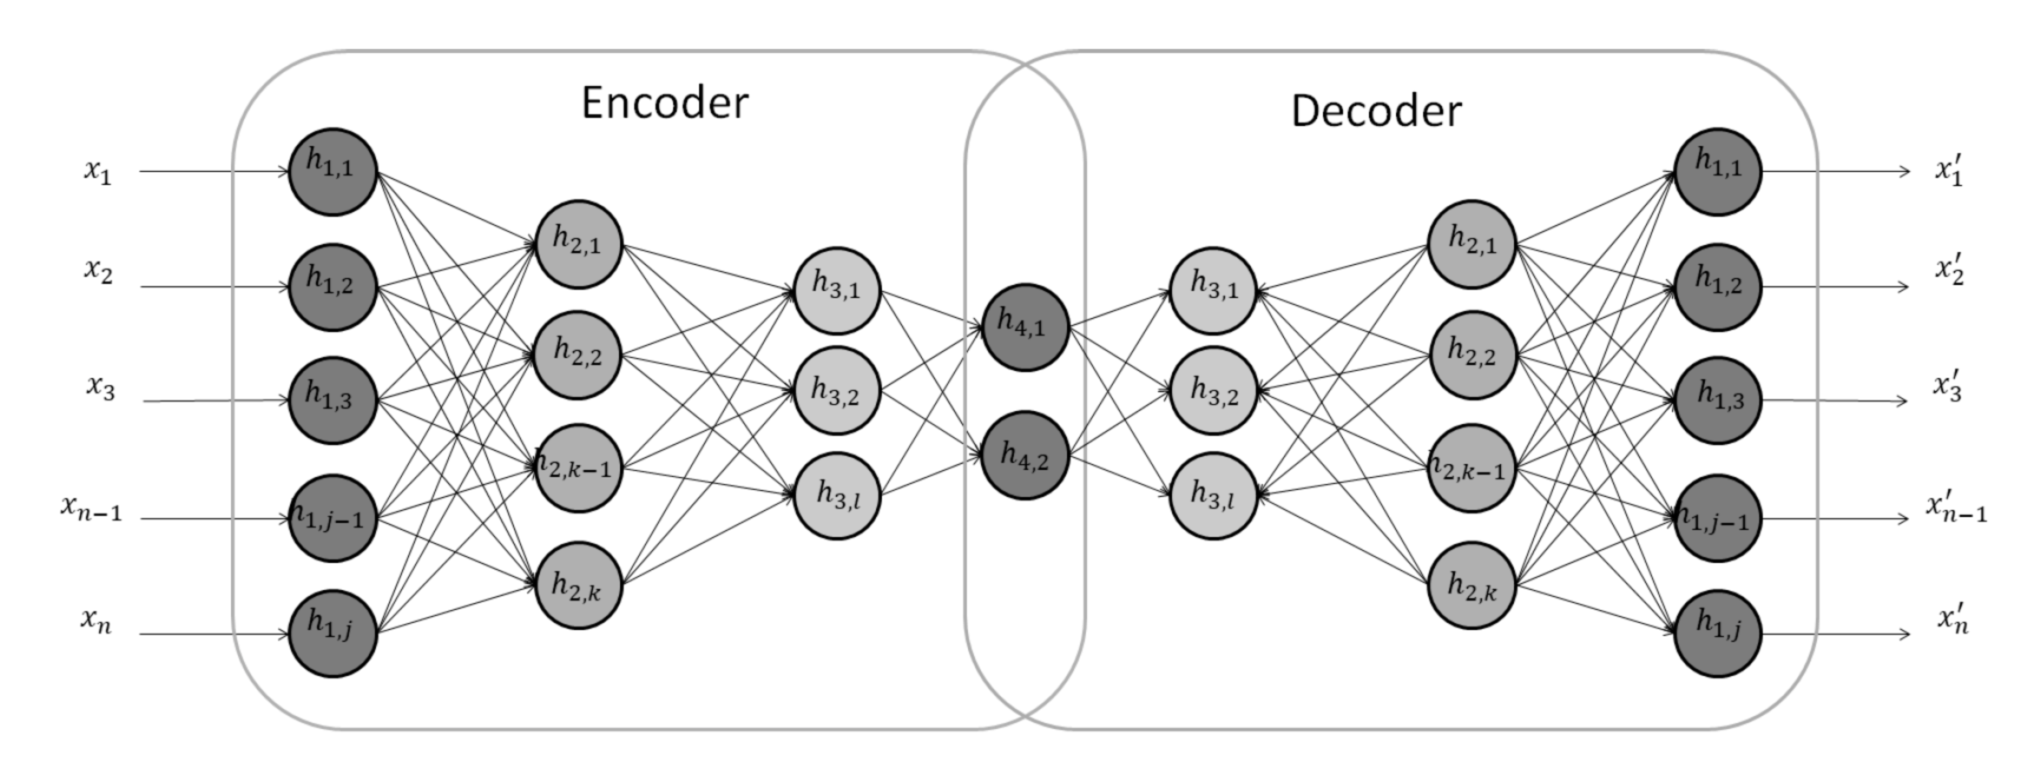
\includegraphics[scale=0.11]{pictures/Auto.PNG}
\caption{Autoencoder}
\label{fig:auto}
\end{figure}

Dimensionality reduction to higher-level features using autoencoders or RBMs with unsupervised extreme machine learning obviously promote the training process of subsequent K-means clustering or classifying for normal/anomaly packets, which is able to fuse semantic information. 

Li, Ma, and Jiao \cite{li2015hybrid} first used an autoencoder to reduce the dimensionality of the data, followed by a DBN with RBM layers that achieved a TPR of 92.2\% with a FPR of 1.58\%. Yousefi-Azar el al. \cite{yousefi2017autoencoder} used an autoencoder with four hidden layers, followed by a Gaussian naive Bayes classifier and achieved an accuracy of 83.34\%. Alom and Taha \cite{alom2017network} implemented both autoencoders and RBMs to perform dimensionality reduction on the KDD-1999 dataset, reducing it to nine features, and then performed K-means clustering on the data, achieving detection accuracies of 91.86\% and 92.12\% accuracy, respectively. 

\subsection{Variant Auto-Encoder}
\label{sec:vae}
Variant Auto-Encoder (VAE) is a specific type of autoencoder but has different purpose. Autoencoder is usually used to extract features by utilizing the encoder part. However, VAE is a generative model which is used to generate data. In VAE, the latent vectors that encoder produces are restricted to a certain distribution such as normal distribution, so that given a sample of normal distribution, the decoder can generate a data in real space. This structure is shown in Fig. \ref{fig:vae}.


\begin{figure}[ht]
\centering
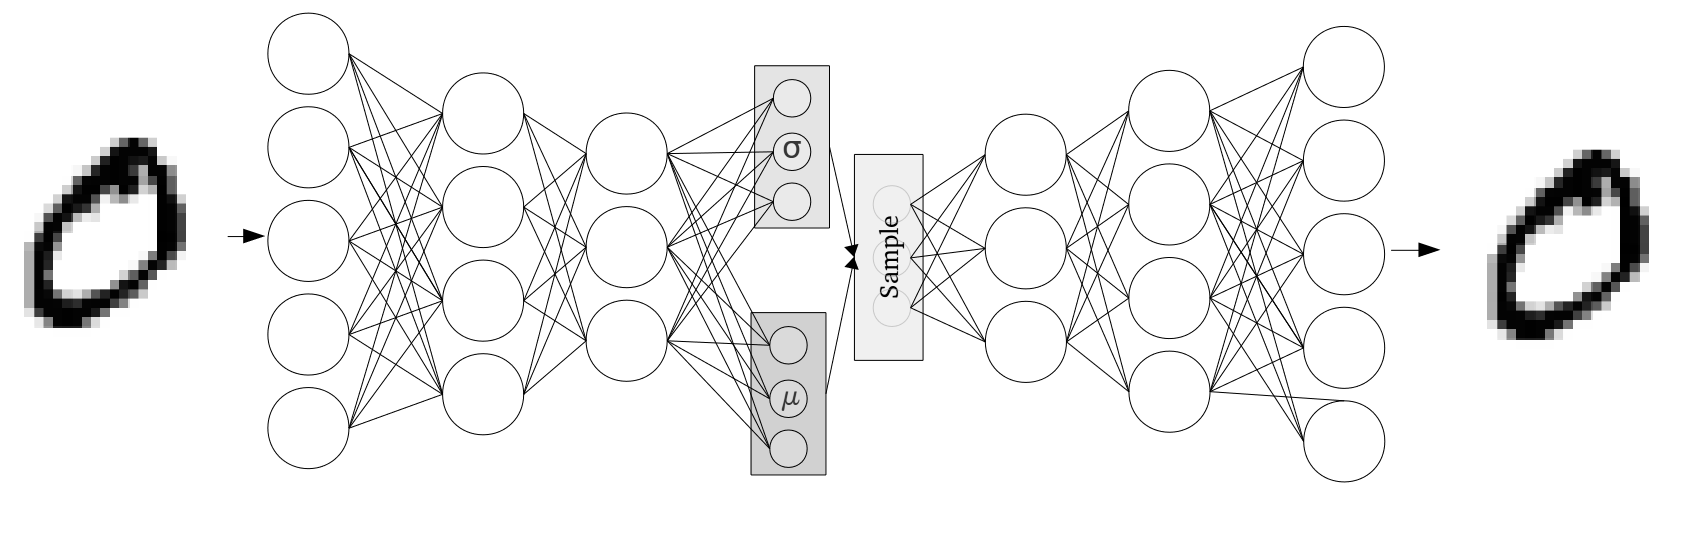
\includegraphics[scale=0.14]{pictures/VAE.png}
\caption{Variant Auto-Encoder}
\label{fig:vae}
\end{figure}

As is shown in Fig. \ref{fig:vae}, the output of encoder is restricted to normal distribution (with mean $\mu$ and standard deviation $\sigma$ ) close to standard normal distribution by minimize formula \ref{vae}. BP can not work because of the sampling operation between encoder and decoder, VAE solves this using reparameterization trick. Once the training finishes, the decoder can be used to generate real data with a sample from standard normal distribution as input.

\begin{equation}
\begin{aligned}
\label{vae}
    K L\left(N\left(\mu, \sigma^{2}\right) \| N(0,1)\right)= \frac{1}{2}\left(\mu^{2}+\sigma^{2}-\log\sigma^{2}-1\right)
\end{aligned}
\end{equation}

As imbalanced dataset, in which anomaly data is far less than normal data, limits the capability of learning methods, synthetic minority reconstruction technique (SMRT) is proposed which uses VAE as a classifier with only the original class distribution. The role of the VAE is to generate synthetic observations of the attack class, which is the minority class, for the sake of handling imbalanced data.

Using the CIDDS-001, Abdulhammed et al. \cite{abdulhammed2019deep} trained a variational autoencoder, a specific type of autoencoder, as well as other machine learning algorithms, to perform intrusion detection, which achieves 97.59\% accuracy, lower than some of the other methods, which were trained using class imbalance correction techniques. The best method was majority voting classifiers, which achieved 99.99\% accuracy. Mirsky et al. \cite{mirsky2018kitsune} created an ensemble of autoencoders, ranging in number from 2 to 48, that were tasked with reconstructing subsets of features, determined using clustering with correlation as the distance metric. The root-mean-square errors (RMSE) of reconstruction from each autoencoder is then used to train a new autoencoder, in which the RMSE represents the anomaly score. Mirsky et al. found that their algorithm performed comparably to or better than algorithms such as isolation forests and Gaussian mixture models.

\subsection{Convolutional Neural Networks}
\label{sec:cnn}
Convolutional neural networks (CNNs) play an important role in recent breakthroughs in computer vision. CNNs are neural networks meant to process input stored in arrays. An example input is an image, which is a 2-dimensional(2D) array of pixels. The architecture of a CNN consists of three distinct types of layers: convolution layers, pooling layers, and the classificaiton layers.


\begin{figure}[ht]
\centering
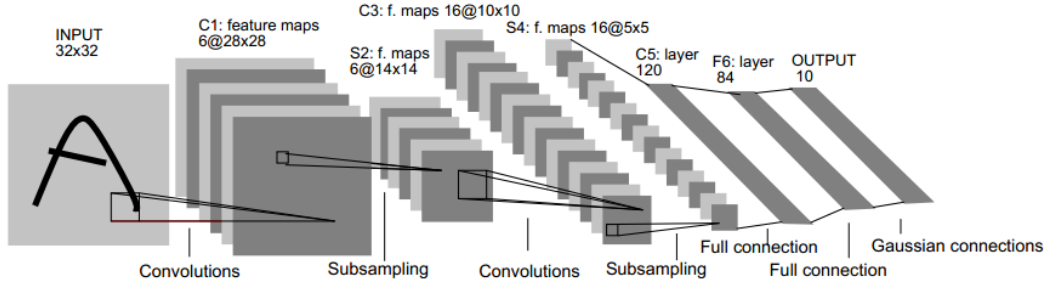
\includegraphics[scale=0.22]{pictures/CNN.PNG}
\caption{Convolutional Neural Network}
\label{fig:cnn}
\end{figure}

Wang et al. \cite{wang2017malware} built an intrusion detection algorithm using raw network traffic data from two existing datasets: the CTU-13 dataset and the IXIA dataset (that the authors called the USTC-TFC2016 dataset), which contained 10 types of normal data and 10 types of malicious data, and appeared to be relatively balanced between malicious and normal. A preprocessing step took the raw network traffic data and converted it into images, which were then fed into a CNN with a similar architecture to the well-established CNN LeNet-5 (LeCun et al. \cite{lecun1995learning}). Because there was no engineering of the preprocessing stage that produced the images, this method handled the raw data directly. The classification was done in two different ways. The first method involved a 20-class classifier, and the goal was to identify which type of normal or malicious the traffic was. The second was a binary classifier which fed into one of two CNNs trained to identify the type of malicious traffic or binary traffic. The 20-class classifier achieved an accuracy of 99.17\%. The binary classifier achieved 100\% whereas the 10-class normal classifier achieved 99.4\% and the 10-class malicious classifier achieved 98.52\%.

% \subsection{Long-Short Term Memory}
\subsection{Recurrent Neural Networks}
Recurrent neural network  (RNNs), extends the capabilities of a traditional neural network, which can only take fixed-length data inputs, to handle input sequences of variable lengths. The RNN can processes inputs one element at a time, using the output of the hidden units as additional input for the next element. Therefore, the RNNs can time series problems such as cyber traffic data.

Standard RNN cannot bridge more than 5–10 time steps.   
Error  signals  tend  to  either  blow-up  or  vanish. 
Blown-up error signals lead straight to oscillating weights, whereas with a vanishing error, learning takes an  unacceptable  amount  of  time,  or  does  not  work at all.  
A detailed theoretical analysis of the problem with long-term dependencies is presented in \cite{hochreiter2001gradient}.  
The paper also briefly outlines several proposals on how to address this problem.

One solution that addresses the vanishing error problem is a gradient-based method called long short-term memory(LSTM) published by \cite{hochreiter1997long}\cite{gers1999learning}\cite{gers2002learning}. LSTM can learn how to bridge minimal time lags of more than 1,000 discrete time steps \cite{hochreiter1997long}.  The solution uses constant error carousels(CECs), which enforce a constant error flow within special cells.  Access to the cells is handled by multiplicative gate units, which learn when to grant access. In the absence of new inputs to the cell, we know that the CEC’s backflow remains constant.  However, as part of a neural  network, the CEC is not only connected to itself, but also to other units in the neural network.  We need to take these additional weighted inputs and outputs into account.  Incoming connections to neuron j can have conflicting weight update signals, because the same weight is used for storing and ignoring inputs.  For weighted output connections from neuron j, the same weights can be used to both retrieve j’s contents and prevent j’s output flow to other neuron s in the network. To address the problem of conflicting weight updates, LSTM extends the CEC with input and output gates connected to the network input layer and to other memory cells.  This results in a more complex LSTM unit, called a memory cell; its standard architecture is shown in Fig \ref{fig:lstm}.

Research results \cite{staudemeyer2015applying}  show that the LSTM classifier provides superior performance in comparison to other tested strong static classifiers. The LSTM classifier shows its strength when training ‘DoS’ attacks and network probes.  The target neuron representing DoS attacks even achieves close to perfect discrimination between attacks and other traffic. These traffic classes tend to generate a high volume of consecutive connection records. Here, LSTM can strongly benefit from the fact that it can look back in time and learn to correlate these connections. So LSTM is very suitable for classifying high-frequency attacks.

\begin{figure}[ht]
\centering
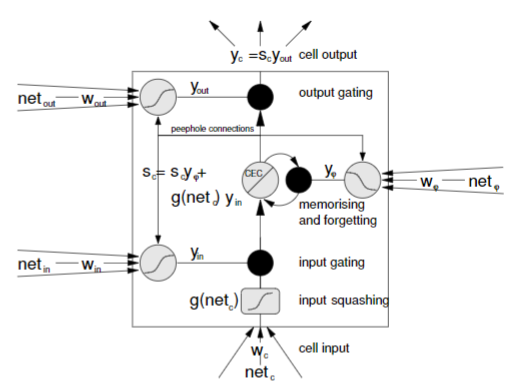
\includegraphics[scale=0.8]{pictures/lstm.png}
\caption{standard LSTM memory cell}
\label{fig:lstm}
\end{figure}

\begin{figure}[ht]
\centering
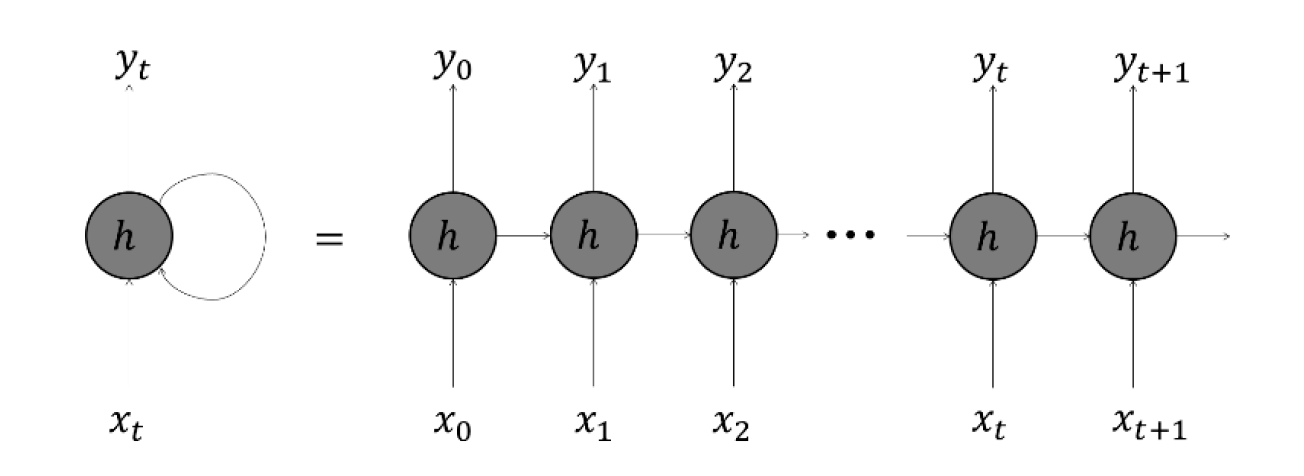
\includegraphics[scale=0.175]{pictures/RNN.PNG}
\caption{Recurrent Neural Network}
\label{fig:rnn}
\end{figure}

\subsection{Generative Adversarial Networks}
\label{sec:gan}
Generative adversarial networks  (GANs), are a type of neural network architecture used in unsupervised machine learning, in which two neural networks compete against each other in a zero-sum game to outsmart each other. One network acts as a generator and another network acts as a discriminator. The generator takes in input data and generates output data with the same characteristics as real data. The discriminator takes in real data and data from the generator and tries to distinguish whether the input is real or fake. When training has finished, the generator is capable of generating new data that is not distinguishable from real data. The generator can learn the distribution of the real data. 

\begin{figure}[ht]
\centering
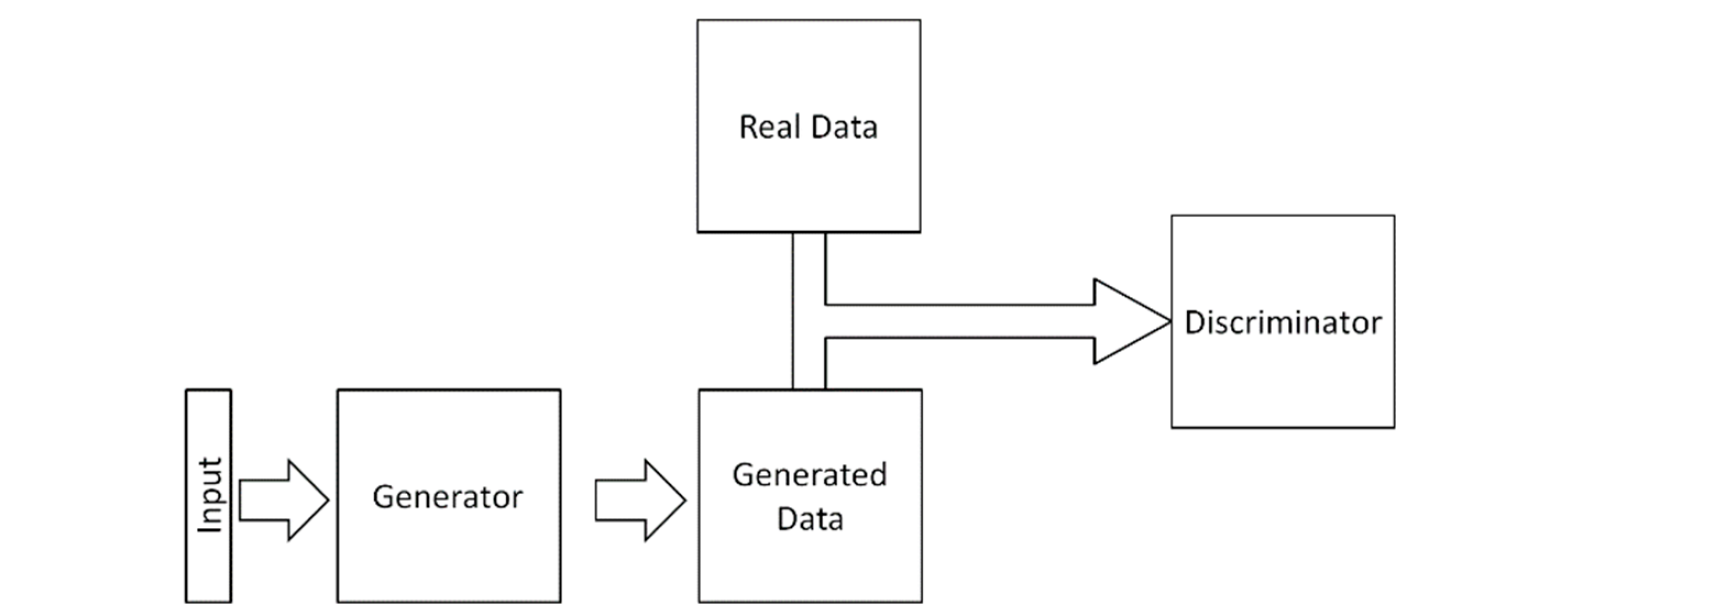
\includegraphics[scale=0.45]{pictures/GAN.PNG}
\caption{Generative Adversarial Network}
\label{fig:gan}
\end{figure}

\begin{figure*}[hbt]
  \centering
  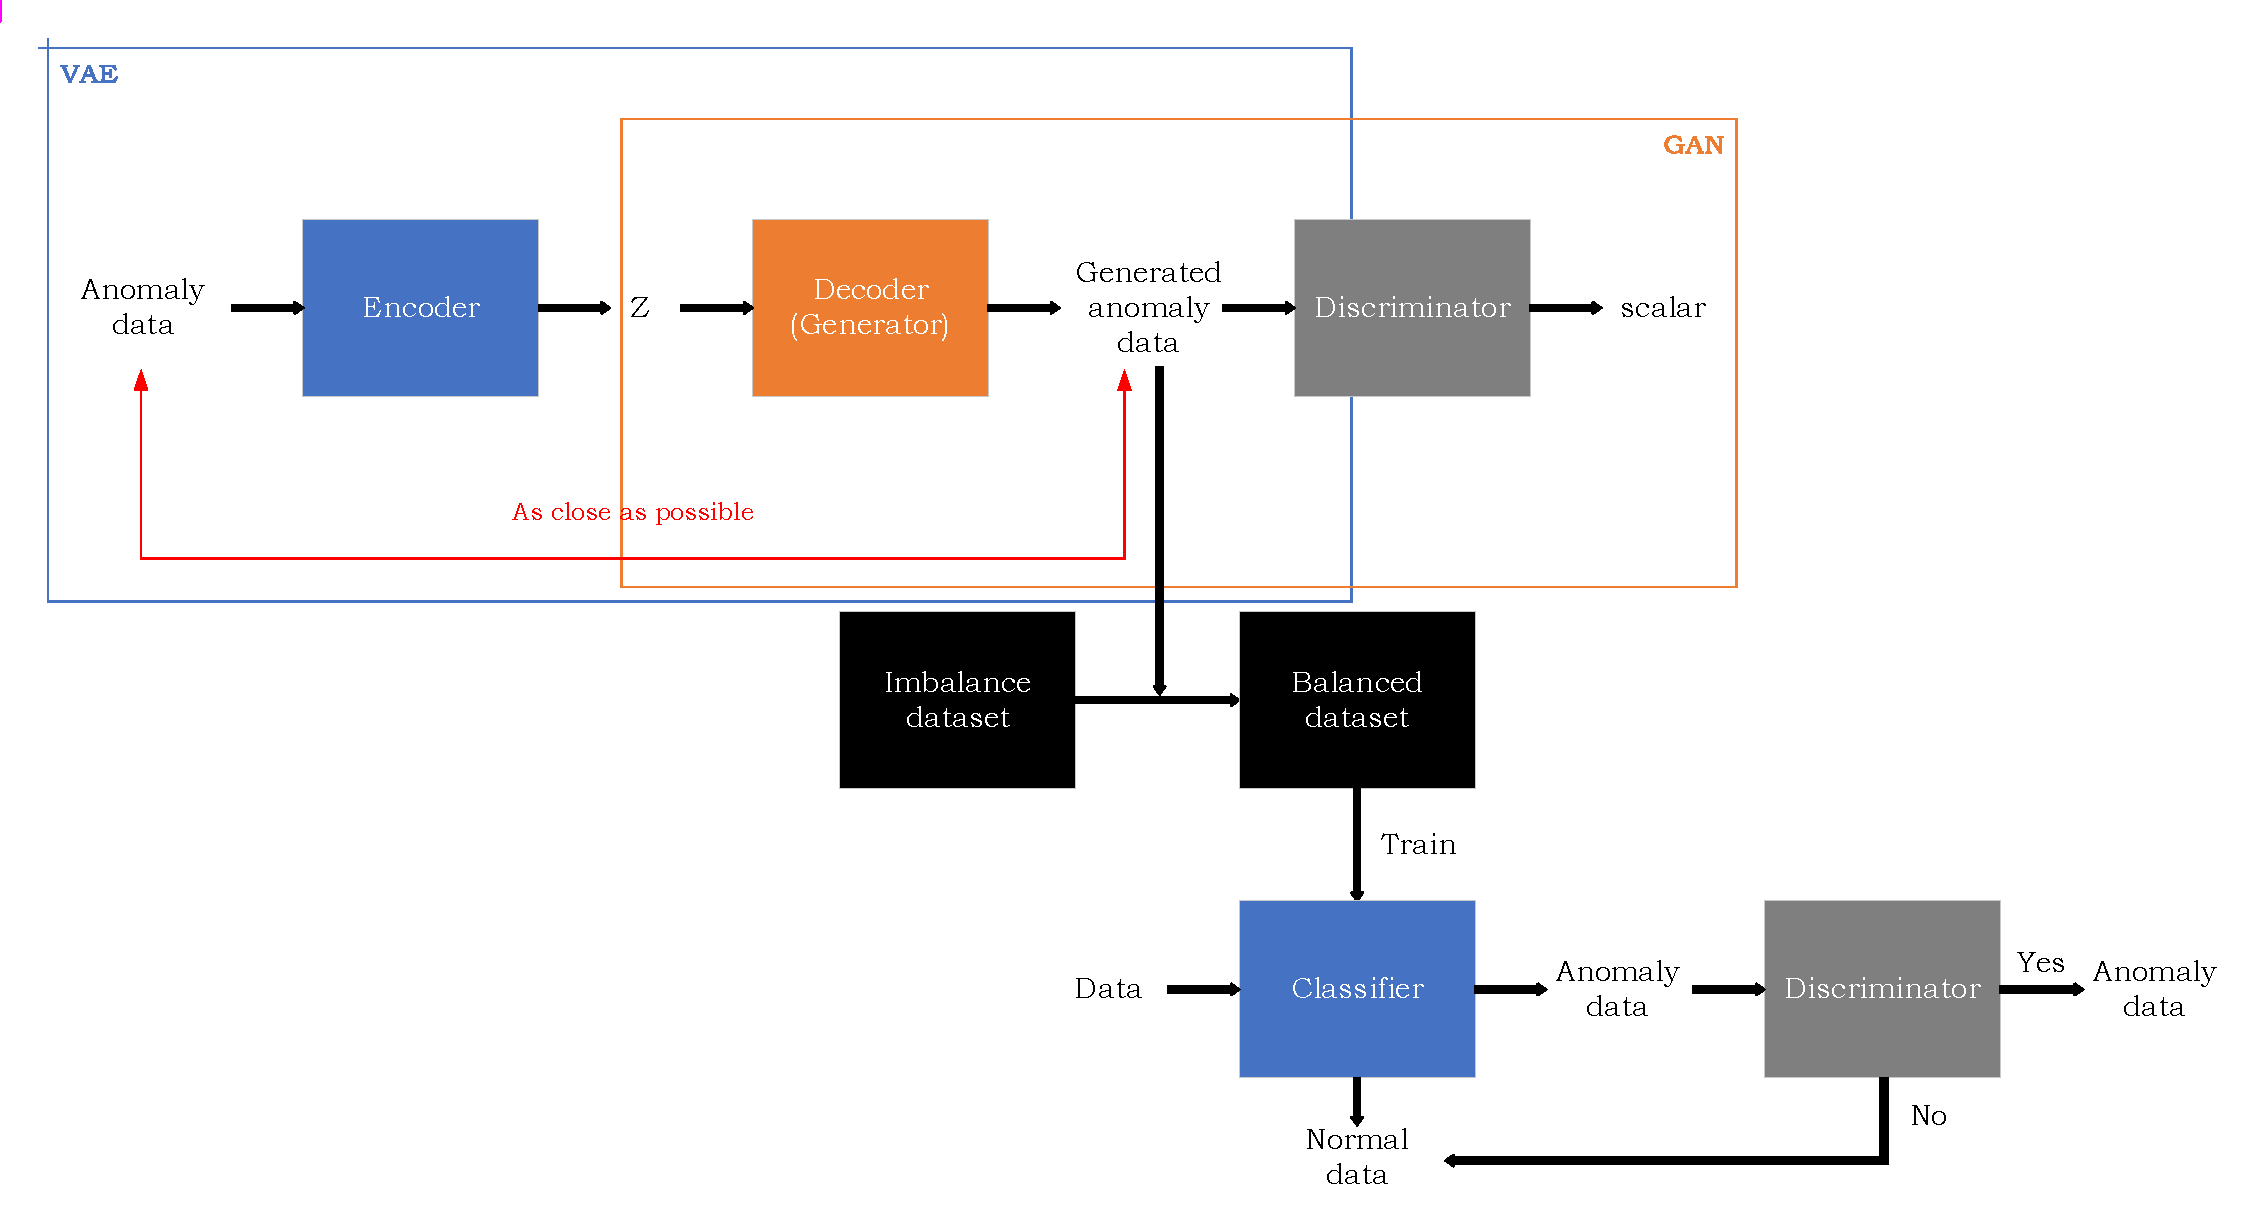
\includegraphics[scale=0.35]{pictures/VAE-GAN-based.pdf}
  \caption{VAE-GAN-based}
  \label{fig:vaegan_base}
  \end{figure*}
In most datasets, anomaly data is far less than normal data. Many methods were proposed to balance the dataset, such as the VAE-based method mentioned in Section \ref{sec:vae}, but GAN-based methods shows a different approach. A GAN can be trained with normal data, so that it learns the distribution of normal data, and the discriminator can be used as a classifier to distinguish anomaly data from normal. AnoGAN\cite{schlegl2017unsupervised} is proposed to better extract
the feature of normal samples, by establishing a mapping between
the real space and latent space. Furthermore, intermediate layer
was introduced in discriminator to optimize the feature extraction. But this mapping is based on the back-propagation algorithm, thus when the dimension of data increases, this model will be timeconsuming and not suitable for timely intrusion detection. To ease the above challenge, a new model \cite{zenati2018efficient} is adopted, inspired by the structure of BiGAN\cite{donahue2016adversarial}, to remarkably reduce the time cost.

However, the following problems remains in the anomaly detection
task. In the training data for cyber-intrusion detection, those discrete features are lethal to traditional GANs, during whose training process the loss criterion is cross-entropy -- a measurement that needs the continuity of features. To overcome the above hurdles, Chen et al.\cite{chen2019gan} proposed a GAN-based model with refined loss function to obtain an outstanding performance on the imbalanced dataset with discrete features. Furthermore, we used the multiple intermediate layers to extract the features in more complex environment.


\section{Prospects}



\subsection{LRCN}


In host system, anomaly traffic can be a serious problem. Suppose a scenario that attackers mix some malicious data into a series of normal packets in a period of time when the terminal is receiving data. Then how to recognize an anomaly packet in a series of packets is really important for system protection. In order to combine temporal information or connections between each packet into the independent features/distribution of one packet, we assume one mechanism to achieve this point. Under this assumption, we can transform a series of data packets into a set of video frames by image generation from traffic data and regard them as a piece of action from outside networks on host.

Deep convolutional neural networks have achieved great success for visual recognition in still images. However, for action recognition in videos, the advantage over traditional methods is not so evident. We aims to design effective ConvNet architectures for action recognition in videos and learn these models given limited training samples by introducing temporal segmentation. 

One succinct preprocessing measure is as follows: First trims or pads all data files to uniform length such as 784 bytes. Then the result can be converted to gray images for every byte range from 0x00 (0) to 0xff (255) representing a pixel. After that they can be analyzed in a visual way. The long-term recurrent convolutional networks (LRCN) framework for proposed by Donahue et al. \cite{donahue2015long} video-based action recognition is based on the idea of long-range temporal structure modeling as shown in Fig. \ref{fig:framework} which combines a sparse temporal sampling strategy and frame series-level supervision to enable efficient and effective learning using the whole normal/intrusion action.

\begin{figure}[ht]
  \centering
  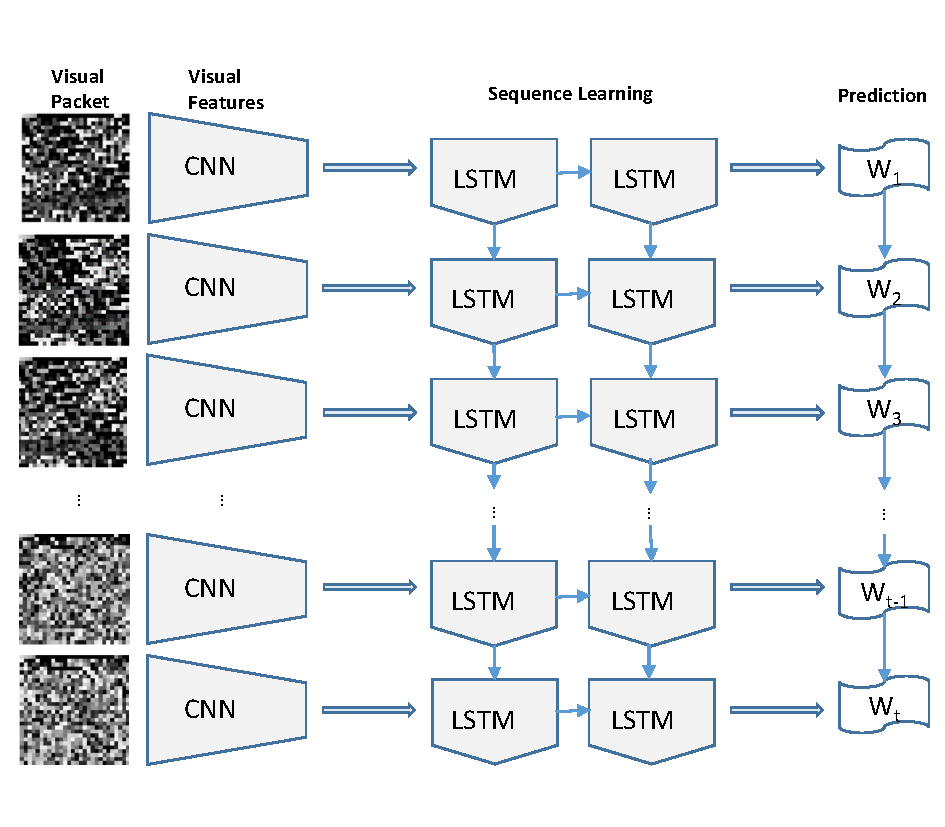
\includegraphics[scale=0.48]{pictures/framework.pdf}
  \caption{Long-term Recurrent Convolutional Networks for traffic classification}
  \label{fig:framework}
  \end{figure}



\subsection{VAE-GAN}
% problems 
Traditional deep learning methods used in NIDS suffer from the problem that the False Detection Rate (FDR) is somewhat high due to the inherent drawback of anomaly detection and the unbalance training data which have much more normal traffic data than abnormal traffic data. The unbalanced category distribution will affect the deep learning model much, specially it will increase false positive rate.

% introduce VAE-GAN (mention that the discriminator can classify 3 classes
% VAE-GAN's effect on solving this problem 1. balance the dataset 2. use classificator and discriminator at the same time .

\begin{figure}[ht]
  \centering
  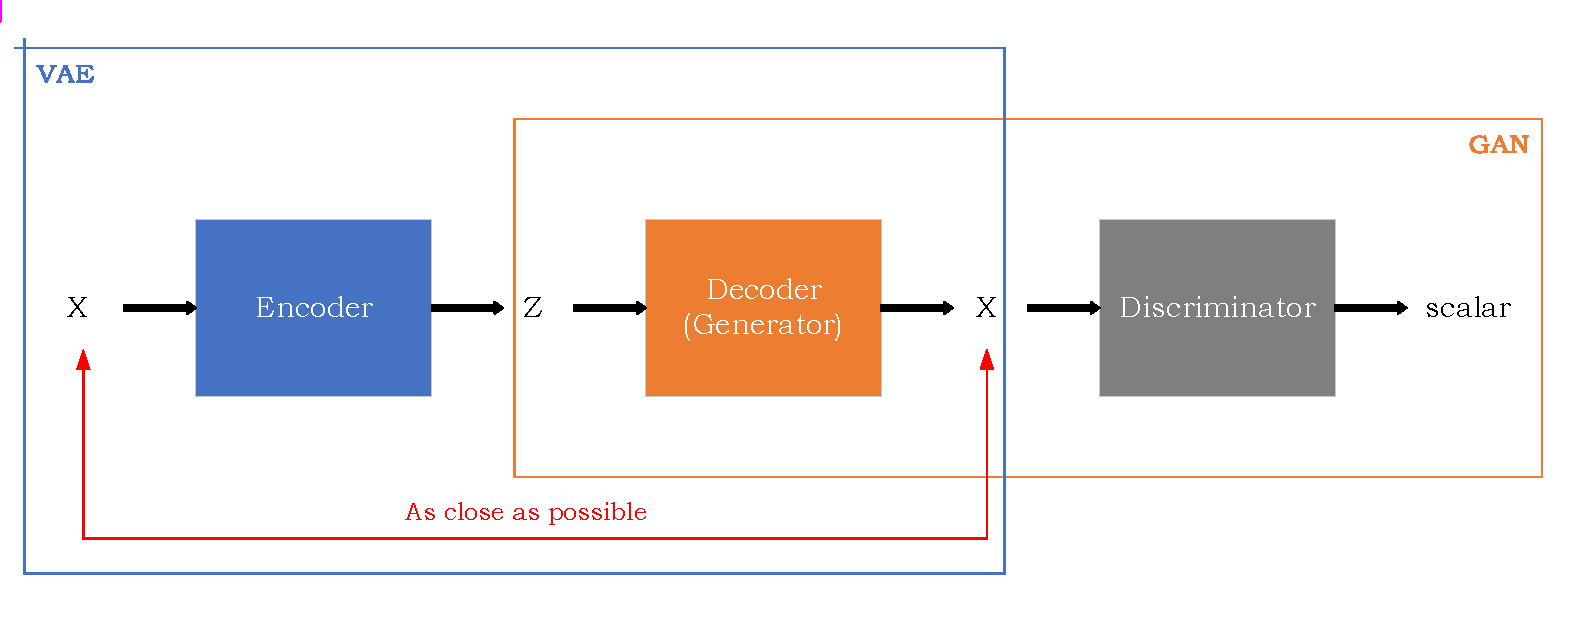
\includegraphics[scale=0.34]{pictures/VAE-GAN.pdf}
  \caption{VAE-GAN}
  \label{fig:vaegan}
  \end{figure}

VAE-GAN is a new model combines VAE(\ref{sec:vae}) and GAN(\ref{sec:gan}), the discriminator learn to discriminate the real($x$), reconstructed($G(E(x))$) and generated($G(z)$) data. 

We can use the decoder (generator) as shown in Fig. \ref{fig:vaegan_base} in VAE-GAN to upsample the minority class of attacking data in datasets instead of using classical VAE, which is more reasonable than Abdulhammed \cite{abdulhammed2019deep} and Mirsky \cite{mirsky2018kitsune} did. Furthermore, there is another profit brought by the well-trained discriminator. After the false detection of anomaly detection (if there are), the discriminator can discriminate the normal packets that classified as intrusion . 



% \subsection{Future Works}
% CNN - more techniques
% GAN - colorful model
% RNN - log auditing
% GNN - graphic flow?

\section{Conclusion}
Protection for a cyber-security system usually lags behind the attacks so intrusion detection plays a significant role in making up the time interval before the reaction of the security system.
The real-time prosperity and scalability are really important. Combining with advances in ML algorithm development offers a rich opportunity to apply neural network-based DL approaches to cyber-security applications to detect new variants of malware and zero-day attacks. Then we aims at keep the networks model time-saving and effective in networks node where lacks computation resources. We give an outline of recent related works in intrusion detection utilized deep learning ways. Different with other surveys or papers, we explore the overview of development by specifically listing the influential works with creative thesis instead of all related works. In future works, the cascading connection of malicious activities throughout an attack lifecycle as we mentioned can be explored to contribute to build an intelligent and efficient networks intrusion detection system. Besides, an idealized framework based on VAE-GAN is designed for processing intrusion detection. 

% Ac is described.NonfVAE-Gerence papers do not normally have an appendix

% use section* for acknowledgment
% \section*{Acknowledgment}


% The authors would like to thank...





% trigger a \newpage just before the given reference
% number - used to balance the columns on the last page
% adjust value as needed - may need to be readjusted if
% the document is modified later
%\IEEEtriggeratref{8}
% The "triggered" command can be changed if desired:
%\IEEEtriggercmd{\enlargethispage{-5in}}

% references section

% can use a bibliography generated by BibTeX as a .bbl file
% BibTeX documentation can be easily obtained at:
% http://mirror.ctan.org/biblio/bibtex/contrib/doc/
% The IEEEtran BibTeX style support page is at:
% http://www.michaelshell.org/tex/ieeetran/bibtex/
%\bibliographystyle{IEEEtran}
% argument is your BibTeX string definitions and bibliography database(s)
%\bibliography{IEEEabrv,../bib/paper}
%
% <OR> manually copy in the resultant .bbl file
% set second argument of \begin to the number of references
% (used to reserve space for the reference number labels box)

\bibliographystyle{IEEEtran}
\bibliography{bibfile.bib}

% \begin{thebibliography}{1}


% \bibitem{IEEEhowto:kopka}
% H.~Kopka and P.~W. Daly, \emph{A Guide to \LaTeX}, 3rd~ed.\hskip 1em plus
%   0.5em minus 0.4em\relax Harlow, England: Addison-Wesley, 1999.

% \end{thebibliography}




% that's all folks
\end{document}


